\documentclass[tikz]{standalone}
\usetikzlibrary{calc}
\usepackage{pgfplots}

\begin{document}


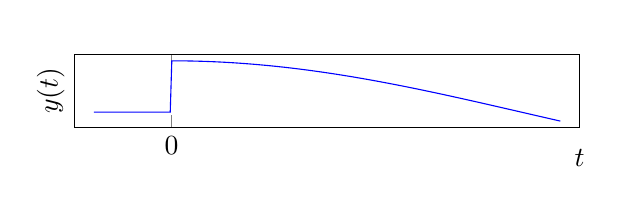
\begin{tikzpicture}
\begin{axis}[ width=8cm,
  height=2.5cm,
  clip=false,
  %xlabel={$t$},
  ylabel={$y(t)$},
  xtick = {0},
  ytick=\empty,
  %xticklabels={$-2h$, $0$, $2h$, $4h$, $6h$, $8h$, $10h$},
  xmin=-2.5,
  xmax=10.5,
]

\addplot+[blue, domain=-2:10, no marks,samples=300,variable=k] { (k>=0)*cos(10*k)}; 

\node at (axis cs: 10.5, -0.9) {$t$}; 
\node[white] at (axis cs: 10.5, 1.3) {$t$}; 
\end{axis}
\end{tikzpicture}
\end{document}
